The distinction between an abstract and concrete workflow instances highlights
an important element of the execution process of a workflow. Abstract workflows
can be interpreted as a formal description of the requirements for the workflow
execution, while concrete workflows can be interpreted as a formal description
of the workflow's execution process. The process of resource selection matches
the resource capabilities to the workflow requirements making possible the
transition from execution requirements to execution process.

Workload managers are those components of workflow systems or, more in general,
of distributed applications that enable resource selection, acquisition, and
use. The set of capabilities required by a workload manager mostly depends on
the heterogeneity and dynamicity of both the workflow and the resources.
Heterogeneity is a measure of the diversity of the workflow requirements and
resource capabilities that need to be matched to enable the execution of the
workflow's tasks; dynamicity is a measure of how much these requirements and
capabilities varies during execution.

The PanDA workload management system was initially designed to manage the
execution of static, relatively homogeneous tasks on dynamic but homogeneous
resources. Progressively, PanDA has evolved to enable the management of more
heterogeneous tasks and resources. In this paper we describe how the design and
architecture of PanDA has enabled executions of multi-threaded tasks on Titan,
currently the largest high performance computing (HPC) resource available in the
USA for scientific research.

Traditionally, the ATLAS workflow has been based on single-core tasks, executed
on Grid resources to process large amount (2TB) of input data divided into
discrete I/O units called ``events''. This approach has many merits: (i)
simplified process of resource selection under the assumption of homogeneous
resources and execution environments; (ii) opportunistic distribution of compute
tasks across resources based on contingent availability; (iii) relative
robustness due to the ability of re-executing failed tasks; and (iv)
multi-tiered distribution and storage of events' data.

Despite all the advantages, ATLAS workflows have evolved to include
compute-intense tasks that can benefit from multithreaded execution on HPC
machines. The Monte Carlo workflow~\cite{} is one of the largest workflows
executed by the ATLAS experiment and at least one of its stages can benefit from
large amount of parallelism. The Geant4 toolkit is used to simulate the passage
of particles through matter and\ldots

\begin{figure}
  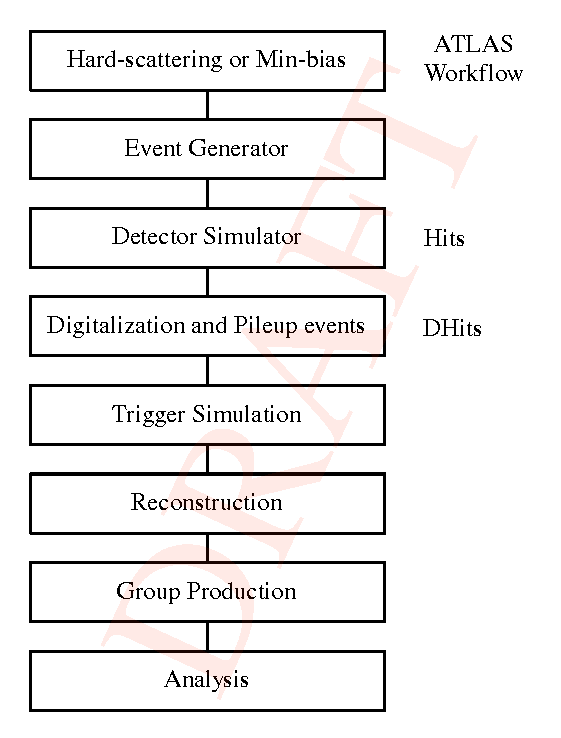
\includegraphics[width=\columnwidth]{figures/atlas_workflow.pdf}
  \caption{ATLAS Monte Carlo workflow.}
\label{fig:atlas_workflow}
\end{figure}

\subsubsection{High-level Description}

\paragraph{Figure~\ref{fig:atlas_workflow} (1)} Multiple end-users (i.e.,
physicists) submit descriptions of ATLAS Monte Carlo Workflows to the JEDI
component of ATLAS middleware. JEDI supervises the execution of these workflows
through a set of eight predefined stages. Each stage requires a specific type of
input and returns a specific type of output. In this paper, we focus on the
third stage called ``Detector Simulator'': the only one, at the moment, executed
on the HPC resources of Titan.

\paragraph{Figure~\ref{fig:atlas_workflow} (2)} JEDI submits/hands over events
to a PANDA Server. This server manages the execution of all the ATLAS workflows
and their stages, including the ATLAS Monte Carlo Workflow. In
Figure~\ref{fig:atlas_workflow} we depicted only how the events of the third
stage are organized within PANDA Server. Tasks are container of jobs and each
job contains itself a set of events. All the events of each job belongs to a
specific submission of a workflow description and, therefore, to a specific user
(i.e., virtual organization). Tasks should therefore be regarded as multitenant
while jobs and their events as monotenant\mtnote{confirmed?}.

\paragraph{Figure~\ref{fig:atlas_workflow} (3)} Sets of events belonging to
multiple tasks and jobs are pushed/pulled? from the PANDA Server to/by one or
more PANDA Pilot. Sixteen? PANDA Pilots are currently instantiated on a
dedicated DSL node of Titan. These instances are responsible for the packaging
of a set of events into a PBS job script. Packaging is performed on the base of
the information gathered about the availability of backfill resources. Depending
on the amount of nodes available, a specific number of events is packaged into
the PBS script.\mtnote{can the events packaged into a PBS job belong to
different submissions and therefore users?}

\paragraph{Figure~\ref{fig:atlas_workflow} (4)} AthenaMP is used to perform the
simulation of the events within the ATLAS detector, 1 AthenaMP thread for each
core available on the Titan nodes. Currently, 16 threads are used for each node,
each thread being able to simulate an average of 1 event every n??
minutes?/second?. So far, no description has been given of the flow of data
required to simulate each event.

Questions for Danila/Sergey:
\begin{itemize}
    \item Does each job of a PANDA Server (and therefore all the tasks of that specific job) belong to the same `user'/VO\@?
    \item Does a PANDA Pilot pull jobs/tasks from a PANDA Server or does a PANDA server push jobs/tasks to a PANDA Pilot?
    \item Does a PANDA Pilot pull jobs or tasks from a PANDA Server? Are the jobs within a PANDA Pilot the same jobs (i.e., the same container of the same tasks) in the PANDA Server?
    \item Do we have 16 PANDA Pilots on a Titan DSL (is this the right acronym?) node? How many DSL nodes?
    \item Can the events packaged into a PBS job belong to different submissions, i.e., different jobs, i.e., different users?
    \item Do we have the distribution of the time taken on titan to process 1 event of the Monte Carlo workflow?
\end{itemize}
